\documentclass[a4paper, 11pt]{article}


% Page Geometry, Typography and Encoding
\usepackage[a4paper, left=2cm, right=2cm, top=2cm, bottom=2.5cm]{geometry} % kleinere Ränder
\usepackage[utf8]{inputenc}
\usepackage[T1]{fontenc}
\usepackage{lmodern} % microtype is not scalable
\renewcommand{\phi}{\varphi}
\renewcommand{\epsilon}{\varepsilon}
% \renewcommand{\theta}{\vartheta} % if you want

% Math packages
\usepackage{amsmath}
\usepackage{amssymb}
\usepackage{amsthm}
\usepackage{mathtools}

% Algorithms and Code
\usepackage{algorithm, caption}
\usepackage{algorithmic}
\usepackage{listings}
\algsetup{indent=1em, linenosize=\tiny}

% Floats
\usepackage{float}
\usepackage{booktabs}
\usepackage{bm}

% Figures
\usepackage{tikz}
\usetikzlibrary{positioning,arrows.meta, patterns, decorations.pathreplacing,calligraphy}
\usepackage{graphicx}
\usepackage{caption}
\usepackage{subcaption}
\usepackage{diagbox} % Diagonal boxes in tabular
\usepackage{collcell}

% Colors
\usepackage{xcolor} %already loaded by tikz, but here for completeness
% RWTH colors
% blue violet purple carmine red magenta orange yellow grass cyan gold silver
\definecolor{rwth-blue}{cmyk}{1,.5,0,0}\colorlet{rwth-lblue}{rwth-blue!50}\colorlet{rwth-llblue}{rwth-blue!25}
\definecolor{rwth-violet}{cmyk}{.6,.6,0,0}\colorlet{rwth-lviolet}{rwth-violet!50}\colorlet{rwth-llviolet}{rwth-violet!25}
\definecolor{rwth-purple}{cmyk}{.7,1,.35,.15}\colorlet{rwth-lpurple}{rwth-purple!50}\colorlet{rwth-llpurple}{rwth-purple!25}
\definecolor{rwth-carmine}{cmyk}{.25,1,.7,.2}\colorlet{rwth-lcarmine}{rwth-carmine!50}\colorlet{rwth-llcarmine}{rwth-carmine!25}
\definecolor{rwth-red}{cmyk}{.15,1,1,0}\colorlet{rwth-lred}{rwth-red!50}\colorlet{rwth-llred}{rwth-red!25}
\definecolor{rwth-magenta}{cmyk}{0,1,.25,0}\colorlet{rwth-lmagenta}{rwth-magenta!50}\colorlet{rwth-llmagenta}{rwth-magenta!25}
\definecolor{rwth-orange}{cmyk}{0,.4,1,0}\colorlet{rwth-lorange}{rwth-orange!50}\colorlet{rwth-llorange}{rwth-orange!25}
\definecolor{rwth-yellow}{cmyk}{0,0,1,0}\colorlet{rwth-lyellow}{rwth-yellow!50}\colorlet{rwth-llyellow}{rwth-yellow!25}
\definecolor{rwth-grass}{cmyk}{.35,0,1,0}\colorlet{rwth-lgrass}{rwth-grass!50}\colorlet{rwth-llgrass}{rwth-grass!25}
\definecolor{rwth-green}{cmyk}{.7,0,1,0}\colorlet{rwth-lgreen}{rwth-green!50}\colorlet{rwth-llgreen}{rwth-green!25}
\definecolor{rwth-cyan}{cmyk}{1,0,.4,0}\colorlet{rwth-lcyan}{rwth-cyan!50}\colorlet{rwth-llcyan}{rwth-cyan!25}
\definecolor{rwth-teal}{cmyk}{1,.3,.5,.3}\colorlet{rwth-lteal}{rwth-teal!50}\colorlet{rwth-llteal}{rwth-teal!25}
\definecolor{rwth-gold}{cmyk}{.35,.46,.7,.35}
\definecolor{rwth-silver}{cmyk}{.39,.31,.32,.14}

% Hyperlinks and Cross-References
\usepackage{hyperref}
\usepackage[capitalise,noabbrev]{cleveref}
\hypersetup{%
	pdftoolbar=false,
	pdfmenubar=false,
	colorlinks,
	%pdfborderstyle={/S/U/W 1.25},
	urlcolor={rwth-magenta},
	linkcolor={rwth-red},
	citecolor={rwth-green}
}

% Programmcode einbetten
\usepackage{listings} %für Code
\usepackage{verbatim} %für mehrzeilige Kommentare
\lstset{literate=
	{Ö}{{\O}}1
	{Ä}{{\A}}1
	{Ü}{{\U}}1
	{ß}{{\ss}}1
	{ü}{{\u}}1
	{ä}{{\a}}1
	{ö}{{\o}}1
}% für Umlaute in Code
\usepackage{xcolor}
\definecolor{codeblue}{rgb}{0,0.6,0.9}
\definecolor{codegray}{rgb}{0.5,0.5,0.5}
\definecolor{codepurple}{rgb}{0.58,0,0.82}
\definecolor{codegreen}{rgb}{0,0.6,0}
\definecolor{codered}{rgb}{0.8,0.2,0}
\definecolor{backcolour}{rgb}{0.96,0.96,0.96}


\lstdefinestyle{mystyle}{
	backgroundcolor=\color{backcolour},   
	commentstyle=\color{codegreen},
	keywordstyle=\color{codeblue},
	numberstyle=\tiny\color{codegray},
	stringstyle=\color{codered},
	emphstyle=\color{codepurple},
	basicstyle=\ttfamily\footnotesize,
	breakatwhitespace=false,         
	breaklines=true,                 
	captionpos=b,                    
	keepspaces=true,                 
	numbers=left,                    
	numbersep=5pt,                  
	showspaces=false,                
	showstringspaces=false,
	showtabs=false,                  
	tabsize=2
}
\lstset{style=mystyle}

 %The min, mid and max values
\newcommand*{\MinNumber}{0.0}%
\newcommand*{\MidNumber}{0.1} %
\newcommand*{\MaxNumber}{1.0}%

%Apply the gradient macro
\newcommand{\ApplyGradient}[1]{%
	\ifdim #1 pt > \MidNumber pt
	\pgfmathsetmacro{\PercentColor}{max(min(100.0*(#1 - \MidNumber)/(\MaxNumber-\MidNumber),100.0),0.00)} %
	\hspace{-0.33em}\colorbox{rwth-blue!\PercentColor!rwth-lblue}{#1}
	\else
	\pgfmathsetmacro{\PercentColor}{max(min(100.0*(\MidNumber - #1)/(\MidNumber-\MinNumber),100.0),0.00)} %
	\hspace{-0.33em}\colorbox{white!\PercentColor!rwth-lblue}{#1}
	\fi
}

\newcolumntype{R}{>{\collectcell\ApplyGradient}c<{\endcollectcell}}
\renewcommand{\arraystretch}{0}
\setlength{\fboxsep}{0.9mm} % box size
\setlength{\tabcolsep}{0pt}

\usepackage{natbib}
\bibliographystyle{plainnat}
\setcitestyle{numbers}
\title{Machine Learning -  Project Report}
\author{Lukas Johannes Ruettgers \and Isaac Hong Zhang Jie \and Chenrui Guo}
\date{\today}

\begin{document}
	\maketitle
	\section{Introduction}
	\section{Reinforcement Learning}
	\subsection{Problem Formulation}
	Reinforcement Learning addresses the problem of learning successful behaviour in an unknown environment. This environment is usually modeled as a stochastic process, namely a \textit{Markov Decision process} (MDP) $(S,A,r,P,\gamma)$. Every process-relevant detail of the environment is included in a state vector $s\in S$, where $S$ is the set of all possible states the environment can be in. The agent has a state-independent set of actions $a\in A$ that describe his options to influence or interact with the environment. The current state $s$ of the environment is usually affected by the action $a$ of the agent, else the action would be useless. 
	The \textit{transition model} $P$ describes how this action changes the environment by providing the new distribution of the states $P(s'\mid s,a)$ after the action was executed. By the Markov assumption, the subsequent state only depends on the prior state and the action and not on states or actions that happened before. Further note that stochastic processes like the MDP regard time as evolving in fixed time steps $t=0,1,\dots$, such that the above term can also be written as $P(s_{t+1}\mid s_t,a_t)$. We however refrained from explicitly denoting the time index in the definition of the transition model $P$ as it might suggest that the transition rule is time-dependent. However, we can consider time-independent transition rules without loss of generality since we can model any time-dependent variables in the state variable $s$ itself. 
	After an action $a$ was executed and led to a new state $s'$, the agent receives a reward $r(s,a,s')$ defined by the reward function $r:S\times A\times S \mapsto \mathbb{R}$. This is the only signal from which the agent can infer what behaviour is desirable. 
	The reinforcement learning problem therefore models learning experience as the experience of state transitions $(s,a,r,s')$, from which the agent shall derive which actions lead in which states to what rewards.
	Na\"ively, we might formulate the objective of the agent as maximizing the expected cumulative reward 
	\[J(a_0,\cdots)=\mathbb{E}_{s_{t+1}\sim P(s_{t+1}\mid s_t,a_t)}\left[\sum_{t=0}^{T-1}r(s_t,a_t,s_{t+1})\right]\]
	over a given \textit{horizon} $T$. However, this objective is ill-defined for an infinite horizon $T=\infty$, where any recurring non-zero reward could accumulate to infinity and render the maximization problem useless. To account for this, a \textit{discount factor} $\gamma\in(0,1)$ is usually used to model the rate with which rewards become more irrelevant over time, such that the objective becomes
	\[J(a_0,\cdots)=\mathbb{E}_{s_{t+1}\sim P(s_{t+1}\mid s_t,a_t)}\left[\sum_{t=0}^{T-1}\gamma^t r(s_t,a_t,s_{t+1})\right].\] 
	A common choice is $\gamma=0.99$, which means that after 100 steps, the reward experienced at the current 100th step is approximately 20 times less important than the very first reward.
	However, this problem formulation is still impractical, since an infinite horizon $T$ will have infinite number of actions as optimization parameters. Instead, we generally describe the behaviour of an agent by a \textit{policy} $\pi(a\mid s)$, which defines a probability distribution over the actions conditioned on each possible state. 
	For a finite number of states and actions, this policy can also be regarded as a lookup table that stores the optimal action distribution in each state. In the case of continuous state domains, this approach renders infeasible and we are left with approximating this function by a set of finite parameters $\theta$.
	Neural network architectures have proven to serve as accurate non-linear function approximators and are widely used in current Deep RL algorithms to approximate $\pi(a\mid s)\approx \pi_\theta(a\mid s)$.
	The objective function then finally writes as
	\begin{align*}
		J(\theta)&=\sum_{t=0}^{T-1}\gamma^t r(s_t,a_t,s_{t+1})\prod_{i=0}^{t}\left(P(s_{i+1}\mid s_i,a_i)\pi_\theta(a_i\mid s_i)\right) \\
		&=\mathbb{E}_{s_{t+1}\sim P(s_{t+1}\mid s_t,a_t),a_t\sim \pi_\theta(a_t\mid s_t)}\left[\sum_{t=0}^{T-1}\gamma^t r(s_t,a_t,s_{t+1})\right].
	\end{align*}
	In the following, we will write $\mathbb{E}_{s_t,a_t\sim \pi_\theta}\left[\cdot \right]$ for notational compactness and to steer the focus on the policy that is to be learnt, while the transition model $p$ is given albeit unknown.
	\subsection{Algorithms and Approaches}
	\subsubsection{Value-based methods}
	The popular methods in classical RL are often categorized as \textit{value-based} and \textit{policy-based} methods. 
	Value-based methods consider the RL problem as a problem of learning the true value of a state $V(s)$ with regard to the expected cumulative reward that is obtainable from it. That is, we define 
	\[V(s)=\mathbb{E}_{s_t,a_t\sim \pi_\theta}\left[\sum_{t=0}^{T-1}\gamma^t r(s_t,a_t,s_{t+1})\mid s_0=s\right].\]
	Similarly, we can further condition this value on the action chosen in this state and obtain a \textit{state-action value}
	\[Q(s,a)=\mathbb{E}_{s'\sim P(s'\mid s,a)}\left[r(s,a,s')+V(s')\right].\]
	If such value functions could be accurately estimated, then an approximately optimal policy could be obtained by deterministically choosing the action that is expected to lead to the states with the highest rewards,
	\[a^{*}=\arg \max_{a\in A}Q(s,a) = \arg \max_{a\in A}\mathbb{E}_{s'\sim P(s'\mid s,a)}\left[r(s,a,s')+V(s')\right],\quad \pi^{*}(a\mid s)=\begin{cases}
		1, & a=a^{*}\\
		0, & a\neq a^{*}\\
	\end{cases}.\]
	The above equality between $V(s)$ and $Q(s,a)$ with regard to optimality in $a$ is known as the \textit{Bellman equation} and paves thFRe way to solving the problem via Dynamic Programming, where an initial estimate $V^{(0)}(s)$ of each state's value is iteratively updated by empirically perceived rewards,
	\[V^{(j+1)}(s)=\max_{a\in A}\mathbb{E}_{s'\sim P(s'\mid s,a)}\left[r(s,a,s')+V(s')\right].\]
	In a similar fashion, $Q(s,a)$ is iteratively updated.
	\subsubsection{Policy-based methods}
	The above schematic algorithm requires executing each action in each state, while the final policy is defined at the end. An alternative approach might include policy behaviour directly from the beginning. That is, we do not update the value functions by executing each possible action and regard them as equally likely, but executing actions with a probability according to a current policy. Because the policy and value functions depend on each other, this paves the way to an iterative update of the policy and the value functions. In the \textit{policy evaluation} step, we firstly update our value functions as
	\[V_\pi^{(j+1)}(s)=\mathbb{E}_{s'\sim P(s'\mid s,a),a\sim \pi(s)}\left[r(s,a,s')+V(s')\right]\]
	for a fixed number of steps or until a convergence criteria is satisfied. Then, we use the updated value functions for \textit{policy improvement} and update $\pi \leftarrow \arg \max_{a\in A}Q_\pi(s,a)$. The repeated iteration over these two processes is called \textit{policy iteration} and often serves as a template for more sophisticated methods.
	Note that the policy that is improved --- the \textit{target policy} --- and the policy that is used for interaction with the environment in the policy evaluation step  --- the \textit{behaviour policy} --- can be different.
	This might be desirable to foster exploration during training, while our final policy should completely exploit the learned knowledge to make the optimal choices. Our current formulation uses the same greedy policy for both steps and hence constitutes an \textit{on-policy} algorithm. But deviating from the target policy with a small probability $\varepsilon\in(0,1)$ and randomly choosing the next action to explore the environment will allow the behaviour policy to escape from local minima and widen its horizon of reward experiences in view of environments that are too high-dimensional or costly too access exhaustively. This \textit{$\varepsilon$-greedy} behaviour policy is the most widely adapted example of an \textit{off-policy} algorithm, but one could also re-use old policies to enrich the learning progress with prior experience. 
	However, both of the formulations above are intractable for infinite state spaces, which we usually face in real-world problems, which requires heuristic approximations in practice.
	\subsubsection{Policy Gradient}
	One alternative viewpoint of the RL problem formulation is to directly regard it as a parametrized optimization problem 
	\[\theta^{*}=\arg\max_{\theta}J(\theta)=\arg\max_{\theta}\mathbb{E}_{s_t,a_t\sim \pi_\theta}\left[\sum_{t=0}^{T-1}\gamma^t r(s_t,a_t,s_{t+1})\right].\]
	To simplify the following notation, we introduce the term \textit{trajectory} $\tau=(s_0,a_0,\dots ,s_T)$ to describe an entire state-action sequence and abbreviate the probability of a trajectory as 
	\[P_{\pi_{\theta}}(\tau)=P(s_0)\prod_{t=0}^{T-1}\pi_\theta(a_t\mid s_t)P(s_{t+1}\mid s_t,a_t),\]
	where $P(s_0)$ is the prior probability distribution of initial states, and define the reward of a trajectory as
	\[r(\tau)=\sum_{t=0}^{T-1}r(s_t,a_t,s_{t+1}).\]
	This way, we streamline the definition of the objective function to
	$J(\theta)=\mathbb{E}_{\tau\sim P_{\pi_{\theta}}}\left[r(\tau)\right]$.
	However, note that this is just a notational simplification. The semantic equality only holds if we multiply the probability of the trajectory from $s_0$ to $s_t$ with the reward \textit{from} $t$ to $T$ and not from $0$ to $T$, where $0\leq t\leq T-1$.
	This imperfection does not matter for the following theoretical analysis in which we can regard the rewards as constants that have been collected during execution in the environment.
	To maximize $J(\theta)$ using gradient ascent, we first have to derive how to compute the gradient; or more specifically, how we compute the gradient of $\pi_\theta(a_t\mid s_t)$, since all other terms are independent of $\theta$.
	Owing to the chain rule, we have the equality
	\[\pi_\theta(a_t\mid s_t)\cdot \nabla\log\left(\pi_\theta(a_t\mid s_t)\right) =  \pi_\theta(a_t\mid s_t)\cdot \frac{1}{\pi_\theta(a_t\mid s_t)} \cdot \nabla \pi_\theta(a_t\mid s_t)=\nabla \pi_\theta(a_t\mid s_t),\quad (PG)\]
	which allows us to obtain the Policy Gradient Theorem
	\begin{align*}
		\nabla J(\theta) &=\nabla \mathbb{E}_{\tau\sim P_{\pi_{\theta}}}\left[r(\tau)\right]\\
		&\overset{\text{Def.}}{=} \nabla \int_{\tau}P_{\pi_{\theta}}(\tau)r(\tau)\,d{\tau}\\
		&\overset{\text{Def.}}{=} \nabla \int_{\tau}\sum_{t=0}^{T-1}\gamma^t r(s_t,a_t,s_{t+1})\prod_{i=0}^{t}\left(P(s_{i+1}\mid s_i,a_i)\pi_\theta(a_i\mid s_i)\right)\,d{\tau}\\
		&\overset{\text{sum rule}}{=} \int_{\tau}\sum_{t=0}^{T-1}\gamma^t r(s_t,a_t,s_{t+1})\nabla \prod_{i=0}^{t}\left(P(s_{i+1}\mid s_i,a_i)\pi_\theta(a_i\mid s_i)\right)\,d{\tau}\\
		&\overset{\text{prod. rule}}{=} \int_{\tau}\sum_{t=0}^{T-1}\gamma^t r(s_t,a_t,s_{t+1})\sum_{j=0}^{t}P(s_{j+1}\mid s_j,a_j)\left(\nabla\pi_\theta(a_j\mid s_j)\right) \prod_{i=0,i\neq j}^{t}\left(P(s_{i+1}\mid s_i,a_i)\pi_\theta(a_i\mid s_i)\right)\,d{\tau}\\
		&\overset{\text{(PG)}}{=} \int_{\tau}\sum_{t=0}^{T-1}\gamma^t r(s_t,a_t,s_{t+1})\sum_{j=0}^{t}\left(\nabla\log\pi_\theta(a_j\mid s_j)\right) \prod_{i=0}^{t}\left(P(s_{i+1}\mid s_i,a_i)\pi_\theta(a_i\mid s_i)\right)\,d{\tau}\\
		&\overset{\text{Def.}}{=} \mathbb{E}_{\tau\sim P_{\pi_{\theta}}}\left[\sum_{t=0}^{T-1}\gamma^t r(s_t,a_t,s_{t+1})\sum_{j=0}^{t}\nabla\log\pi_\theta(a_j\mid s_j)\right]\\
		&\overset{\text{rearrange}}{=} \mathbb{E}_{\tau\sim P_{\pi_{\theta}}}\left[\sum_{j=0}^{T-1}\nabla\log\pi_\theta(a_j\mid s_j) \sum_{t=j}^{T-1}\gamma^t r(s_j,a_j,s_{j+1})\right]\\
		&\overset{T\to\infty}{=} \mathbb{E}_{\tau\sim P_{\pi_{\theta}}}\left[\sum_{j=0}^{\infty}\nabla\log\pi_\theta(a_j\mid s_j) Q_{\pi_{\theta}}(s_j,a_j)\right].
	\end{align*}
	The benefit of this transformation is that we reduced computing the gradient of an expectation value over the rewards to the expectation value of a policy gradient term. Even though the rigorous exact computation remains intractable for infinite or high-dimensional state and action spaces, we can avail to common strategies in Inference Statistics to estimate this expectation value given only few samples of the entire population of possible trajectories.
	That is, one could for example collect $N$ trajectories at each gradient ascent step and approximate the estimation value of the $\log$ terms as the arithmetic mean of the $\log$ terms over these $N$ trajectories, as is done in classical \textit{Monte Carlo} RL. This is the approach that the REINFORCE algorithm takes, which belongs to one of the first algorithms in the category of policy gradient methods.
	To further alleviate the computation of the $\log$ term itself, REINFORCE approximates $\pi(a\mid s)$ as a normal Gaussian probability distribution. While the mean of this distribution is estimated using a neural network $\mu \approx f_\theta(s)$, the covariance matrix is often heuristically fixed as $\Sigma$.
	This way, we have
	\[\pi_\theta(a_t\mid s_t)=\frac{1}{\sqrt{(2\pi)^n|\Sigma|}}\exp\left(-\frac{1}{2}(f_{\theta}(s_t)-a_t)\Sigma^{-1}(f_{\theta}(s_t)-a_t)\right), \text{ and consequently}\]
	\[\log\pi_\theta(a_t\mid s_t)=\log\left(\frac{1}{\sqrt{(2\pi)^n|\Sigma|}}\right)  -\frac{1}{2}(f_{\theta}(s_t)-a_t)\Sigma^{-1}(f_{\theta}(s_t)-a_t).\]
	Because the first term is constant with regard to $\theta$, this finally yields us the gradient
	\[\nabla\log\pi_\theta(a_t\mid s_t)=-\Sigma^{-1}(f_{\theta}(s_t)-a_t)\frac{\partial f_\theta}{\partial \theta}.\]
	As all activation functions in today's neural network architectures are differentiable, $\frac{\partial f_\theta}{\partial \theta}$ is simply obtained for each weight $\theta_i$ by the back-propagation algorithm. The pseudocode for REINFORCE is depicted below in Figure \ref{fig:reinforce}.
	
	\begin{figure}[H]
		\begin{algorithm}[H]
			\caption{\textbf{REINFORCE}}
			\small % Adjust font size
			\raggedright
			\renewcommand{\algorithmicrequire}{\textbf{Initialize:}} % Set name of subalgorithm
			\begin{algorithmic}[1]
				\REQUIRE{Neural network $\pi_\theta$ with parameters $\theta$, learning rate $\alpha$, covariance matrix $\Sigma$, batch size $N$.}
				\WHILE{not converged}
				\STATE{Collect $N$ trajectories $(s_0,a_0,r_0,\dots, s_T)$ by executing $\pi_\theta$ and store them in a buffer $B$.}
				\FORALL{trajectories $\tau$ in $B$}
				\FORALL{transitions $(s_t,a_t,r_t)\in\tau$}
				\STATE{Forward $s_t$ through $\pi_\theta$ to obtain the distribution $\pi_\theta(a_t\mid s_t)$.}
				\STATE{Track the gradient history to obtain $\nabla\log\pi_\theta(a_t\mid s_t)=-\Sigma^{-1}(f_{\theta}(s_t)-a_t)\frac{\partial f_\theta}{\partial \theta}$.}
				\STATE{Run the BP algorithm to update $\theta \leftarrow \theta + \alpha \cdot \nabla\log\left(\pi_\theta(a_t\mid s_t)\right)r_t$.}
				\ENDFOR
				\ENDFOR
				\ENDWHILE
			\end{algorithmic}
		\end{algorithm}
		\caption{REINFORCE pseudo code algorithm.}
		\label{fig:reinforce}
	\end{figure}
	
	As for normal Monte-Carlo RL methods, the estimation on long-horizon trajectories exhibit a huge variance, because the domain of possible state-action combinations grows exponentially in the horizon $T$.
	On the other side, the \textit{Temporal Difference} update 
	\[V^{(j+1)}(s)=V^{(j)}(s)+\alpha \left(r(s,a,s')+\gamma V^{(j)}(s')-V^{(j)}(s)\right),\]
	which considers only one transition with empirical reward in the update of the value function, has a low variance. But it has a larger bias, which comes from the larger weight estimate of the value $V(s_{t+1})$ of the subsequent state, which was only discounted once by the discount rate $\gamma$. 
	To mitigate the variance while preserving a low bias, an unbiased baseline can be subtracted from the rewards. The value function $V_{\pi_{\theta}}(s)$ turns out to be such a good baseline, resulting in the adjusted term 
	\[J(\theta)=\mathbb{E}_{\tau\sim P_{\pi_{\theta}}}\left[\sum_{j=0}^{\infty}\nabla\log\pi_\theta(a_j\mid s_j) \left(Q_{\pi_{\theta}}(s_j,a_j)-V_{\pi_{\theta}}(s)\right)\right].\]
	This term is also known as the \textit{advantage function} $A_{\pi_{\theta}}(s_t,a_t):=Q_{\pi_{\theta}}(s_t,a_t)-V_{\pi_{\theta}}(s)$, which measures the advantage, when taking action $a_t$ over alternative actions in $s_t$ and continuing to act by the policy $\pi_{\theta}$. If the rewards perceived in this trajectory are high, then $a_t$ truly exhibits an advantage over the average action, because $V(s_t)$ is defined as the \textit{expectation value} of cumulative rewards.
	To approximate this advantage function with a good trade-off between Temporal Difference with low variance and Monte Carlo with low bias, one could theoretically choose any $1\leq n \leq T$, accumulate the empirical rewards until step $n$ and cap off with the prior estimate of the value function at the $n$-th state,
	\[V^{(j+1)}(s_t)=A_n(s_t,a_t):=\sum_{i=0}^{T-1}\left(\gamma^i r(s_{t+i},a_{t+i},s_{t+i+1})\right) +\gamma^n V^{(j)}(s_{t+n})-V^{(j)}(s_t).\]
	This term $A_n(s_t,a_t)$ is often referred to as the $n$-step approximation of the \textit{advantage function}.
	The \textit{Generalized Advantage Estimation} combines all these terms into one and steers their importance decay with one hyperparameter $\lambda\in(0,1)$, culminating in
	\[A_{GAE}(s_t,a_t)=\frac{1}{1-\lambda}\sum_{n=1}^{T}\lambda^n A_n(s_t,a_t)=\frac{1}{1-\lambda}\sum_{i=0}^{T}(\lambda\gamma)^i\left( r(s_{t+i},a_{t+i},s_{t+i+1}+\gamma V(s_{t+i+1})-V(s_{t+i})\right).\]
	
	\subsubsection{Proximal Policy Optimization}
	There are also numerous other optimization techniques to improve the objective function $J(\theta)$. To unravel this bouquet of opportunities, consider an alternative parametrization $\theta'$. The \textit{Performance Difference Lemma}, whose proof follows a similar spirit as the one for the Policy Gradient Theorem, states that 
	\[J(\theta')-J(\theta)=\mathbb{E}_{\tau\sim P_{\pi_{\theta'}}}\left[\sum_{t=0}^{\infty} A_{\pi_{\theta}}(s_t,a_t) \right].\]
	Intuitively, this means that $\theta'$ is desirable over $\theta$ if the new policy $\pi_{\theta'}$ executes those actions with a higher probability that are advantageous even if we follow the old policy $\pi_{\theta}$ in the subsequent states. Unfortunately, the evaluation of this term requires an approximation of the distribution of states and actions under the very $\theta'$ that we are trying to optimize. Na\"ively, this would require to empirically estimate the distribution under $P_{\pi_{\theta'}}$ with a large number of trajectories for each $\theta'$ we want to consider as a new parameter candidate, which imposes a severe computational limitation on the number of $\theta'$s that one can explore in each update step.
	Instead we can constrain $\theta'$ to remain close to $\theta$ with regard to $P_{\pi_{\theta}}$. Then approximating 
	\[\mathbb{E}_{\tau\sim P_{\pi_{\theta'}}}\left[\sum_{t=0}^{\infty} A_{\pi_{\theta}}(s_t,a_t) \right]\approx\mathbb{E}_{\tau\sim P_{\pi_{\theta}}}\left[\sum_{t=0}^{\infty} \frac{\pi_{\theta'}(a_t\mid s_t)}{\pi_{\theta}(a_t\mid s_t)}A_{\pi_{\theta}}(s_t,a_t) \right]\]
	will not exhibit a large distributional shift in the likelihood of states. \textit{Trust Region Policy Optimization} formulates this as a constrained optimization problem and maximize
	\[J(\theta')=\mathbb{E}_{\tau\sim P_{\pi_{\theta}}}\left[\sum_{t=0}^{\infty} \frac{\pi_{\theta'}(a_t\mid s_t)}{\pi_{\theta}(a_t\mid s_t)}A_{\pi_{\theta}}(s_t,a_t) - \delta \operatorname{KL}\left(\pi_{\theta}(a_t\mid s_t)||\pi_{\theta'}(a_t\mid s_t)\right) \right],\]
	which can be solved by conjugate gradient algorithm that however requires second-order derivatives to approximate the penalty KL divergence term. Instead, \textit{Proximal Policy Optimization} proposes a first-order approximation 
	\[J(\theta')=\mathbb{E}_{\tau\sim P_{\pi_{\theta}}}\left[\sum_{t=0}^{\infty} \min\left(1+\varepsilon,\frac{\pi_{\theta'}(a_t\mid s_t)}{\pi_{\theta}(a_t\mid s_t)}\right)A_{\pi_{\theta}}(s_t,a_t)\right]\]
	that clips overly advantageous deviations from the current policy $\pi_{\theta}$ and therefore evokes a more stable, stepwise optimization procedure. Since the estimation of the advantage function requires a state-value function $V$, a separate neural network is trained as \textit{critic}. Together with the critic loss and a term that encourages entropy on the action distribution of $\pi_{\theta'}(a_t\mid s_t)$, the above $J(\theta')$ constitute the loss function $J(\theta',\psi')$. The original paper trains multiple agents in parallel (\cite{schulman2017proximal}), but since it is no specific feature of PPO, we omitted it in the pseudocode in Figure \ref{fig:ppo}.
	\begin{figure}[H]
		\begin{algorithm}[H]
			\caption{\textbf{Proximal Policy Optimization}}
			\small % Adjust font size
			\raggedright
			\renewcommand{\algorithmicrequire}{\textbf{Initialize:}} % Set name of subalgorithm
			\begin{algorithmic}[1]
				\REQUIRE{Actor network $\pi_\theta$, value network $V_{\psi}$, clip offset $\varepsilon$, scaling coefficients $c_1,c_2$ for entropy and value loss, batch size $N$, training epochs $K$, minibatch size $M$.}
				\WHILE{not converged}
				\STATE{Collect $T$ transitions $(s_t,a_t,r_t,s_{t+1})$ by executing $\pi_\theta$ and store them in a buffer $B$.}
				\STATE{Compute advantage estimators $\hat{A}_{\pi_{\theta}}^{(i)}$ for each transition $1 \leq i \leq T$.}
				\FOR{epoch $1\leq j\leq K$}
				\FORALL{transitions $(s_t,a_t,r_t,s_{t+1})$ in minibatch of size $M$}
				\STATE{Optimize $\theta'$ and $\psi'$ with regard to $J(\theta',\psi')$.}
				\ENDFOR
				\STATE{Update $\theta \leftarrow \theta',\psi\leftarrow \psi'$}
				\ENDFOR
				\ENDWHILE
			\end{algorithmic}
		\end{algorithm}
		\caption{PPO pseudo code algorithm.}
		\label{fig:ppo}
	\end{figure}
	\section{Experiment Setup}
	\subsection{Experiment Objective}
	In this experiment, we want to investigate the performance of both PPO and REINFORCE on the \texttt{LunarLander-v2} environment provided by OpenAI's \texttt{gymnasium} package. We seek to understand how sensitive the model's performance is to some hyperparameters, which are concretized in the following.
	For PPO, we alternate over
	\begin{itemize}
		\item three different reward configurations, which mainly deviate in sparsity,
		\item the learning rates $\alpha=0.01,0.001,0.0003$ to validate whether faster rates than the low default learning rate of $3e-4$ still achieve stable training progress,
		\item the discount factors $\gamma=0.5,0.7,0.999$ to compare far more shortsighted with the default, quite longsighted agent with $\gamma=0.999$, and
		\item the clip offsets $\varepsilon=0.1,0.2,0.3$ as suggested by the original paper \cite{schulman2017proximal} to impose different restrictions on the policy's freedom to profit from its advantages.
	\end{itemize}
	The experiments for PPO were not done in parallel, but sequentially, and the best hyperparameters in each earlier experiment were fixed for the subsequent experiments.
	For REINFORCE, we alternate over
	% TODO: Specific experiment values.
	\begin{itemize}
		\item the Generalized Advantage Estimation discount $\lambda$
		\item the learning rate $\alpha$,
		\item the discount factor $\gamma$ to compare shortsighted with more longsighted agents, and
		\item the batch size $N$
	\end{itemize}
	\subsection{LunarLander Environment}
	The lunar environment simulates the problem of landing a spacecraft on a platform. The observation space $(q_x,q_y,\vartheta,v_x,v_y,\omega,\ell,r)$ is quasi-continuous and comprises both the robots coordinates, azimuthal angle, linear and angular velocities and two boolean variables that reflect if the left or right leg contact point touched the land.
	The actions space is finite and merely continue four actions:
	\begin{itemize}
		\item Action 0: Do nothing,
		\item Action 1: Fire left orientation engine,
		\item Action 2: Fire the main engine,
		\item Action 3: Fire right orientation engine.
	\end{itemize}
	
	\subsection{Rewards}
	We use different reward configurations during training. The first is the default reward configuration, which is fine-tuned and hence provides an accurate, dense signal towards the goal region. Specifically, the reward after an action
	\begin{itemize}
	\item is increased/decreased the closer/further the lander is to the landing pad,
	\item is increased/decreased the slower/faster the lander is moving,
	\item is decreased the more the lander is tilted (angle not horizontal),
	\item is increased by 10 points for each leg that is in contact with the ground,
	\item is decreased by 0.3 points each frame the main engine is firing,
	\item is decreased by 0.03 points for each side engine firing,
	\item is increased by 100 points for landing safely, and
	\item is decreased by 100 points for crashing.
	\end{itemize}
	The reward configuration in the task description of our course project instead awards 100 points for each leg making ground contact and thus incentives safe landing. It also slight penalizes usage of the main engine to promote fuel efficiency. This approach allows for a nuanced modification of the reward system, encouraging behaviors like safe landing and fuel efficiency while still adhering to the game's fundamental objectives.
	We refer to this reward configuration as the \textit{custom} reward, which --- for completeness ---
	\begin{itemize}
	\item is increased by 100 points for each leg that is in contact with the ground,
	\item is decreased by 0.3 points each frame the main engine is firing,
	\item is increased by 100 points for landing safely, and
	\item is decreased by 100 points for crashing.
	\end{itemize}
	
	To firstly showcase the relevance of the omitted rewards and secondly study how the higher leg contact reward affects the learning performance, we finally extend the custom reward by all terms that were not included. For the terms that are already included, we leave the values the same and do not adjust them to the values from the default reward configuration. Specifically, this leads to a \textit{combined} reward that deviates only from the default reward in assigning not 10 but 100 points for each leg contact.
	\subsection{Implementation}
	\subsubsection{PPO}
	To ensure a correct implementation of PPO, we availed to the PPO implementation of \texttt{Stable Baselines 3}. 
	Each model is trained for 1,500,000 iterations, which amounts to 367 policy updates and evaluations. While the model was only trained on one vectorized environment for simplicity, it was evaluated on 10 different environment configurations to obtain a more general evaluation score. Evaluation of the model's mean reward was done after every four policy updates. After training has finished, the model's mean reward was evaluated one final time.
	The implementation is available in a Jupyter Notebook which was supplied along with the report.
	The CustomCallback subclass of the BaseCallback class provides the mean rewards in training and evaluation mode for each episode, which were collected and finally plotted together.
	\subsubsection{REINFORCE}
	% TODO: Implementation Details.
	\subsubsection{Reproducibility}
	To ensure the reproducibility of the experiment results, all pseudorandom number generators from torch, numpy or the internal random package were fixed. Moreover, we tried to force torch and CUDA to use only deterministic algorithms by setting the environment variable \texttt{CUBLAS\_WORKSPACE\_CONFIG} according to the API Reference Guide of cuBLAS \cite{Nvid.CUDA}. However, we weren't able to perform any operations on the GPU if we set this variable. 
	Since some of the models themselves already exhibited variance, we decided to run the experiments on a CPU and not a GPU to clearly distinguish variance that emerges from GPU operations from the variance inherent to the model architecture.
	In the experiments with Stable Baselines 3, we however still observed small variances in the learning curves of agents with the exact same configuration. However, this variance was small and eventually does not perturb our results.
	\section{Experiment Results}
	\subsection{PPO}
	\begin{figure}[H]
		\begin{center}
		\begin{subfigure}{0.48\textwidth}
			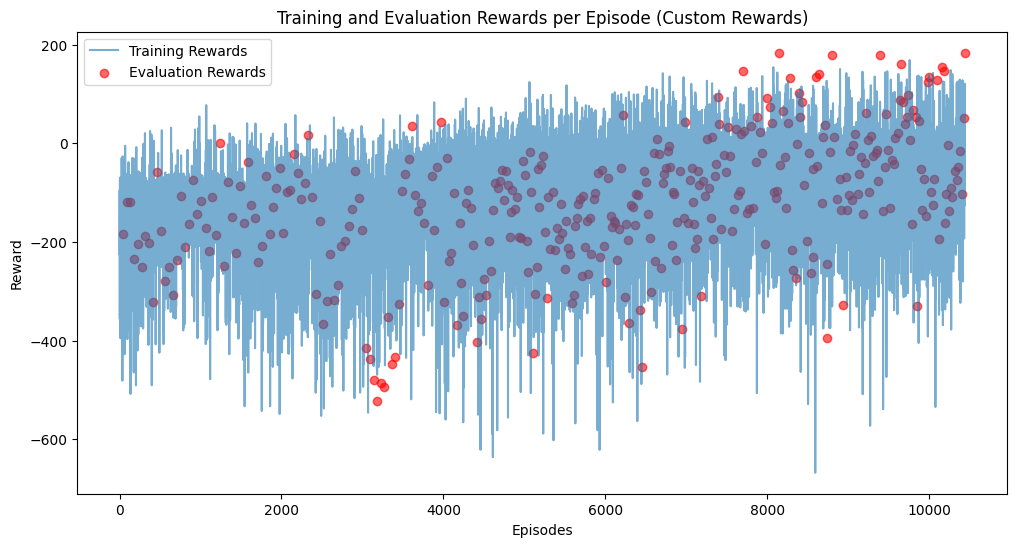
\includegraphics[width=\linewidth]{ppo_figures/custom_env_results.png}
			\caption{Project-custom rewards}
			\label{fig:ppo_rewcust}
		\end{subfigure}\hfill 
		\begin{subfigure}{0.48\textwidth}
		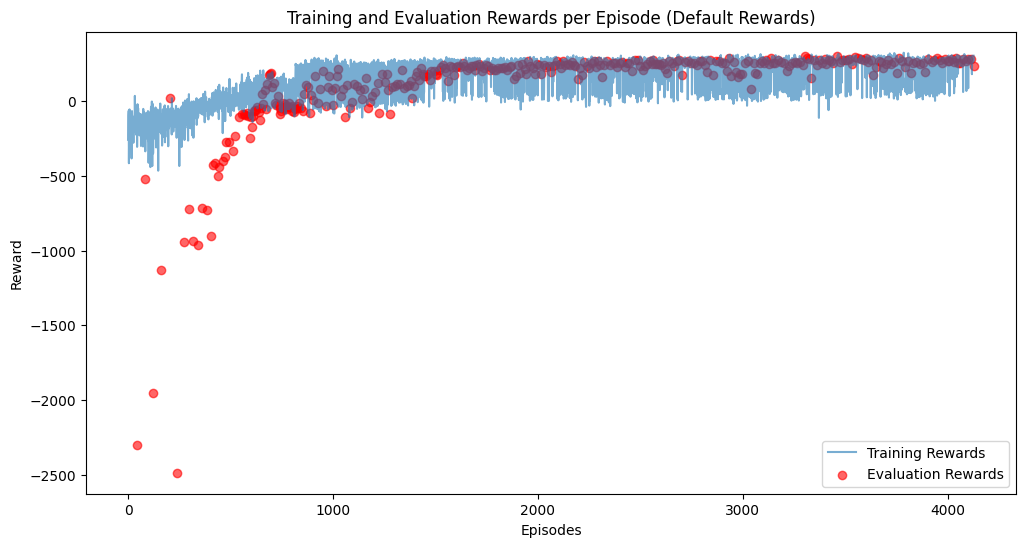
\includegraphics[width=\linewidth]{ppo_figures/default_env_results.png}
		\caption{Default rewards}
		\label{fig:ppo_rewdef}
		\end{subfigure}\\ 
		\begin{subfigure}{0.48\textwidth}
		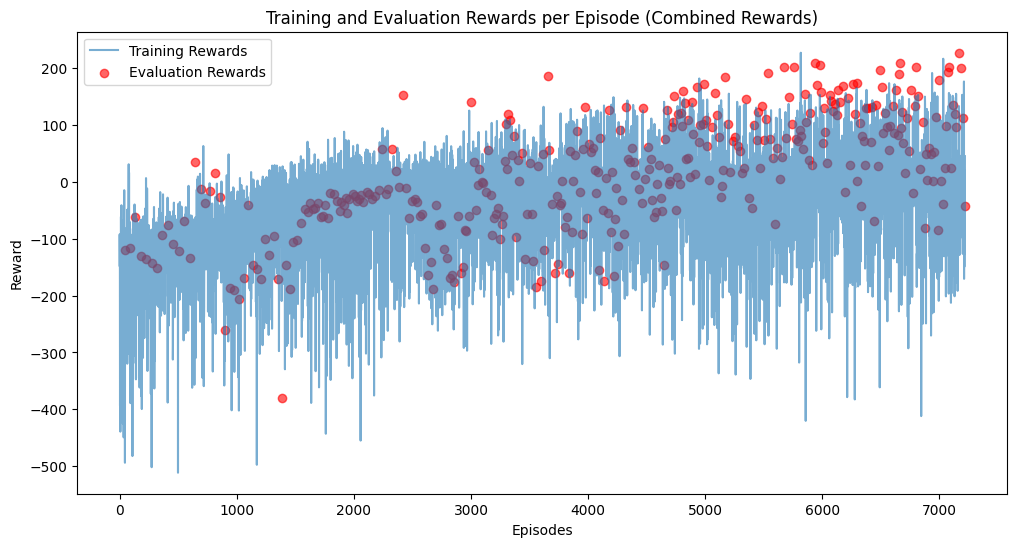
\includegraphics[width=\linewidth]{ppo_figures/combined_env_results.png}
		\caption{Combined rewards}
		\label{fig:ppo_rewcomb}
		\end{subfigure}
	\end{center}
		\caption{Training and evaluation rewards of PPO for different reward configurations, namely the custom reward configuration proposed in the course project description, the default reward configuration of the environment, and a combination of both.}
		\label{fig:ppo_reward}
	\end{figure}
	In the custom reward configuration, the agent will only receive any positive signal at the very end of the landing process, that is when a leg touches the ground and the overall landing process was successful. Before, it will only receive negative rewards for activating the main engine. Moreover, there is neither punishment nor reward for using the side engines. The agent actions will therefore obtain two degrees of freedoms on these two actions and result in uncontrolled, randomized behaviour with overwhelming probability.
	This exacerbates the ability to learn stable successful long-horizon behaviour, as the intermediate steps taken do not directly receive any feedback. Conversely, the default reward configuration provides a dense training signal that rewards the agent for any improvement in the distance between the landing unit and the spacecraft, which quickly steers the agent into the region of interest where he then perceives rich reward experience. As the comparison in Figure \ref{fig:ppo_rewcust} demonstrates, the custom rewards exhibit a huge variance, because the agent lacks reward signals that teach him a fine-granular usage of his engines and will not acquire a stable behaviour. Conversely, the agent that perceives the default rewards converges faster and more stable to successful behaviour (Fig. \ref{fig:ppo_rewdef}), although its variance is only slightly smaller than the variance of the agent with the custom rewards. The quite negative rewards at the first evaluations scale the figure to a far larger range and creates the wrong illusion that the variance decreased drastically. For the combined model where only the positive reward for leg contact was enlarged from 10 to 100, the variance remains similar to the agent with the default rewards (Fig. \ref{fig:ppo_rewcomb}). However, it fails to live up to the average final reward of around 150 of the default reward agent, since it oscillates rather around 110 during the final evaluations. 
	For each of the three models, we have provided evaluation videos in the \texttt{ppo\_eval\_videos} folder. While the model with the default rewards succeeds in all final evaluation runs, the model with combined rewards only succeeds in half of them and the model with the custom rewards in almost none.
	The evaluation video of the model with custom rewards illustrates the uncontrolled usage of the side engines stressed in the experiment setup section. Although the model even has a quite fortunate initial force applied that pushes it directly to the landing area without requiring usage of the side engines, the model starts to activate the side engines in a seemingly uncontrolled way and drafts to the left.
	What's more, the model with the combined rewards seems to continue using the side engines although it has already landed in the goal area, as our example evaluation video illustrates. This behaviour is particularly odd since the model even receives a small punishment for using the side engines. We believe it might be due to a bug in the environment which does not regard the agent's position as goal state and refrains from terminating the run, such that our model tries to trigger the termination by hovering over the landing area.
	Nevertheless, this behaviour did not occur for the model with the default rewards, which only changed in the smaller reward scale for leg contact with the ground.
	This proves how brittle the reward function can become from small deviations from a fine-tuned superposition and underscores the importance of providing a dense reward signal to stabilise the optimization procedure.
	For the following, we hence continued with the default reward configuration.
	
	\begin{figure}[H]
		\begin{center}
			\begin{subfigure}{0.48\textwidth}
				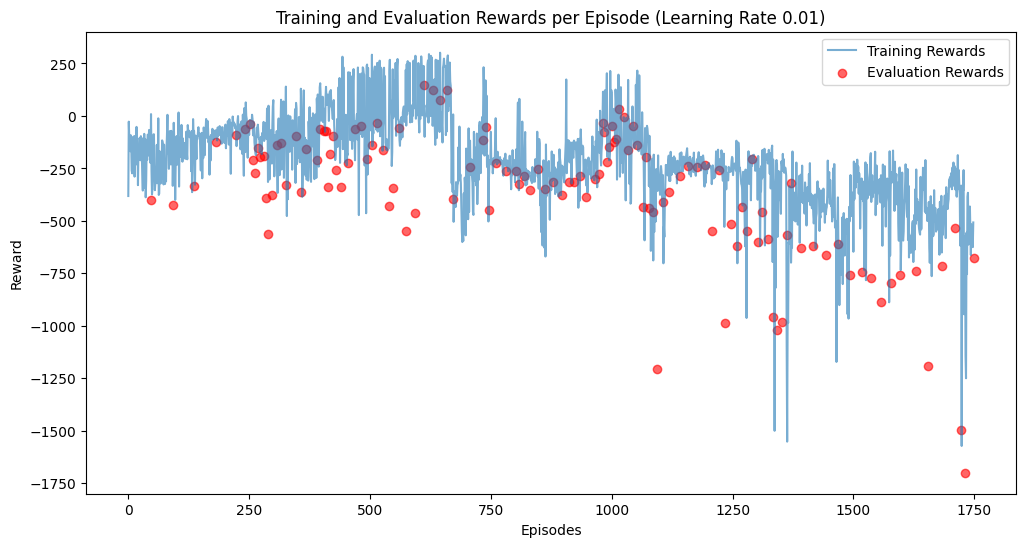
\includegraphics[width=\linewidth]{ppo_figures/lr_results_0.01.png}
				\caption{$\alpha=0.01$}
				\label{fig:ppo_lr0.01}
			\end{subfigure}\hfill 
			\begin{subfigure}{0.48\textwidth}
				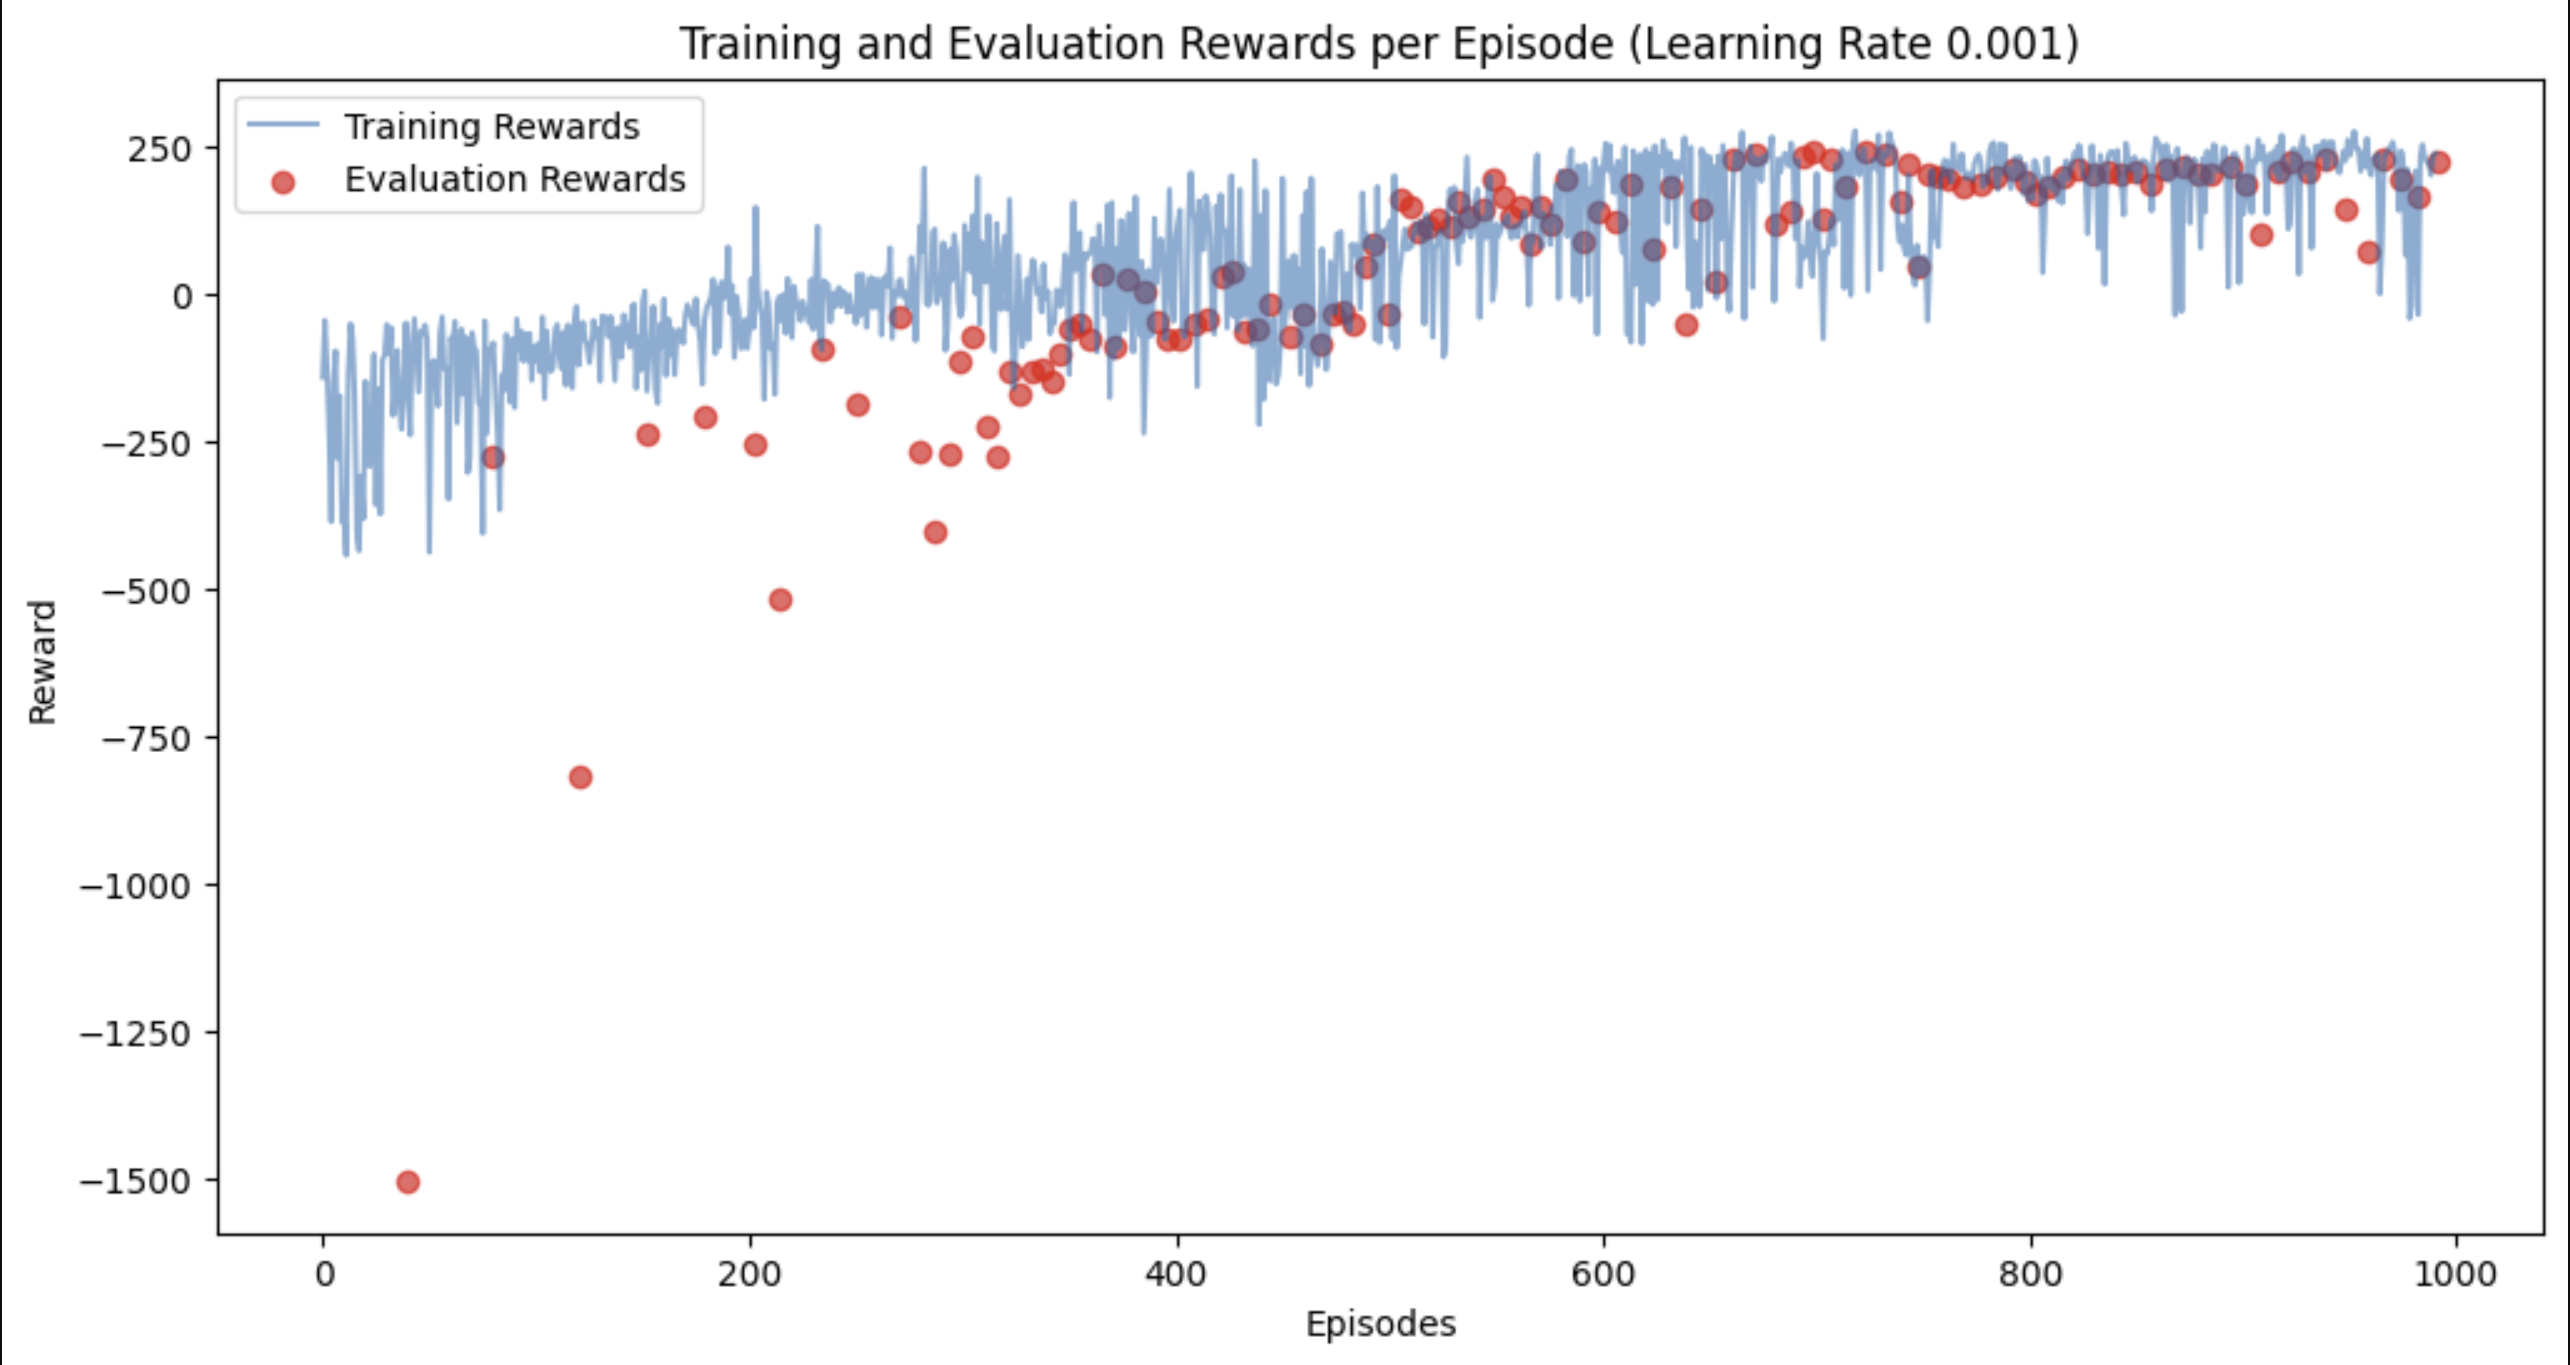
\includegraphics[width=\linewidth]{ppo_figures/lr_results_0.001.png}
				\caption{$\alpha=0.001$}
				\label{fig:ppo_lr0.001}
			\end{subfigure}\\
			\begin{subfigure}{0.48\textwidth}
				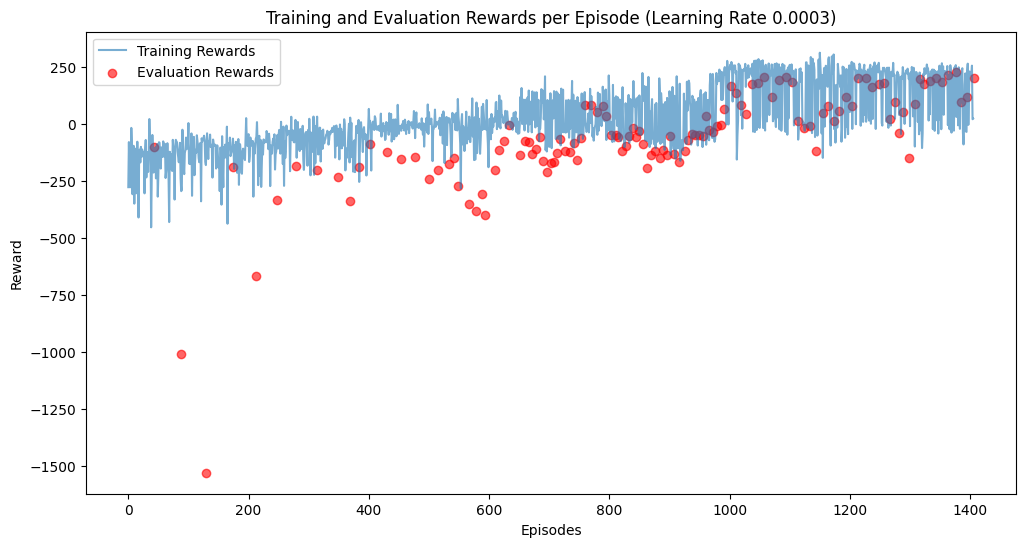
\includegraphics[width=\linewidth]{ppo_figures/lr_results_0.0003.png}
				\caption{$\alpha=0.0003$}
				\label{fig:ppo_lr0.0003}
			\end{subfigure} 
		\end{center}
		\caption{Training and evaluation rewards of PPO for different learning rates $\alpha=0.01,0.001,0.0003$.}
		\label{fig:ppo_lr}
	\end{figure}
	The default learning rate of $\alpha=0.0003$ slowly approaches a sound mean reward (Fig. \ref{fig:ppo_lr0.0003}), but interestingly exhibits more variance during training and evaluation than the agent with the slightly larger learning rate of $\alpha=0.001$ (Fig. \ref{fig:ppo_lr0.001}). Originally, we expected the opposite behaviour, since a smaller learning rate should slow down the overall parameter change and hence the change in behaviour. What we did not consider in the beginning is that the behaviour itself can exhibit a large variance in performance due to imperfect actions.
	We hypothesize that the slightly larger learning rate allows the optimization process to easier escape from local minima and converge faster to stable and successful performance. Especially at the end, both the training and evaluation mean reward achieve an unparalleled stability in a high value range of more than 150 (Fig. \ref{fig:ppo_lr0.001}).
	On the contrary, the slower parameter changes for $\alpha=0.0003$ might prolong the required training time for culminating in successful behaviour. This reminds us of the importance of choosing the learning rate not too small as it might be less robust to a function landscape with many local minima. On the other hand, Fig. \ref{fig:ppo_lr0.01} illustrates that convergence can not be guaranteed for higher learning rates and in our case eventually leads to divergence. The agent fails to acquire any improvement in the policy and never settles down in a good solution region.
	We therefore continue our experiments with $\alpha=0.001$.
	
	\begin{figure}[H]
	\begin{center}
		\begin{subfigure}{0.48\textwidth}
			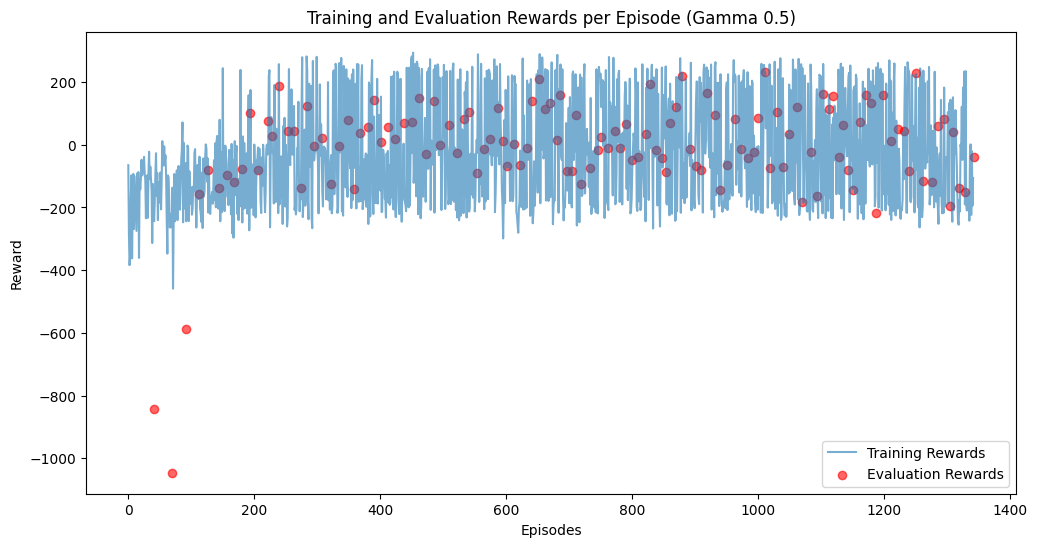
\includegraphics[width=\linewidth]{ppo_figures/gamma_results_0.5.png}
			\caption{$\gamma=0.5$}
			\label{fig:ppo_gamma0.5}
		\end{subfigure}\hfill 
		\begin{subfigure}{0.48\textwidth}
		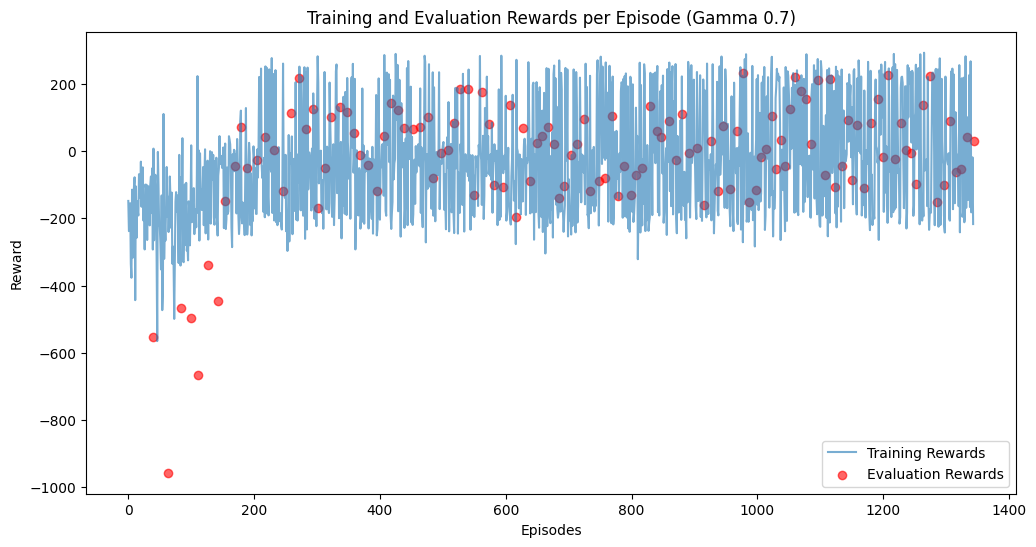
\includegraphics[width=\linewidth]{ppo_figures/gamma_results_0.7.png}
		\caption{$\gamma=0.7$}
		\label{fig:ppo_gamma0.7}
		\end{subfigure}\\
		\begin{subfigure}{0.48\textwidth}
		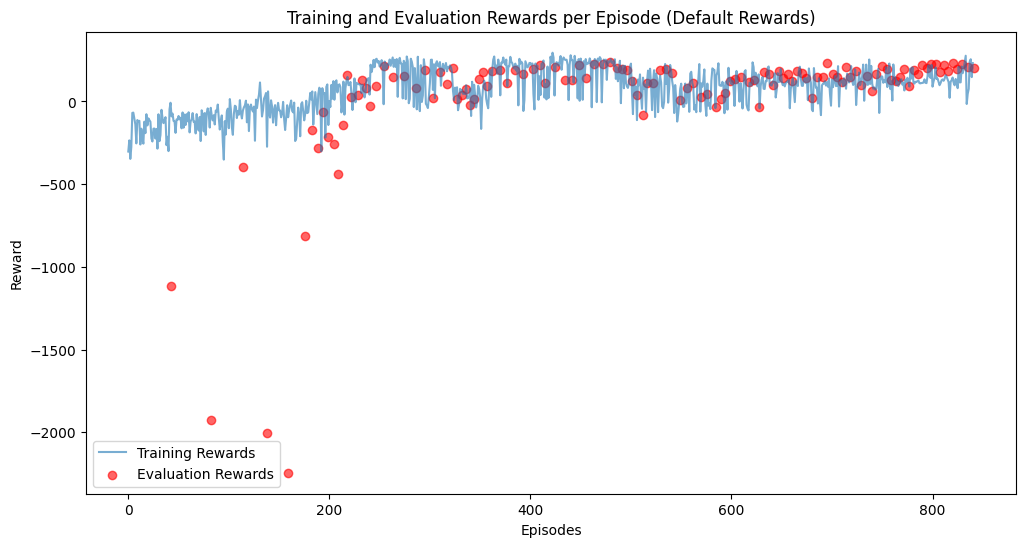
\includegraphics[width=\linewidth]{ppo_figures/gamma_results_0.9.png}
		\caption{$\gamma=0.999$}
		\label{fig:ppo_gamma0.999}
		\end{subfigure}
	\end{center}
	\caption{Training and evaluation rewards of PPO for different discount rates $\gamma=0.5,0.7,0.999$.}
	\label{fig:ppo_gamma}
	\end{figure}
	
	To end up stably on the ground, the spacecraft has to go through more than multiple dozens of actions and understand long-term physical relations between the change in position and velocity due to activations of the main and side engines.
	The default high discount rate of $\gamma=0.999$ implies a quite farsighted agent, which still weighs rewards perceived after 100 steps with a weight of 0.9 and will hence allow the terminal reward signals of successful landing or leg contact to effect actions made far earlier.
	In general, a sufficiently high discount rate is necessary to allow the agent to understand long-range causations. The agent with this high learning rate has the same configuration as the agent from the earlier Figure \ref{fig:ppo_lr0.001}, but obtains even more stable results due to randomness we could not fix during the training process. On the other hand, an agent with $\gamma=0.7$ will result in a cumulative discount of around 3\% after only 10 steps, while the agent with $\gamma=0.5$ even reaches $0.1$\%. As mentioned before, this prohibits the agent from comprehending the long-term impacts of engine activations on the dynamics of the space craft and hinders him from obtaining stable behaviour as Figures \ref{fig:ppo_gamma0.5} and \ref{fig:ppo_gamma0.7} depict. The discount factor depends both on the reward scale and the usual trajectory horizon and clearly profits from a high value of $\gamma=0.999$, while $\gamma=0.99$ might be a better choice for other environments. 
	Here, we stick with $\gamma=0.999$.
	
	\begin{figure}[H]
		\begin{center}
			\begin{subfigure}{0.48\textwidth}
				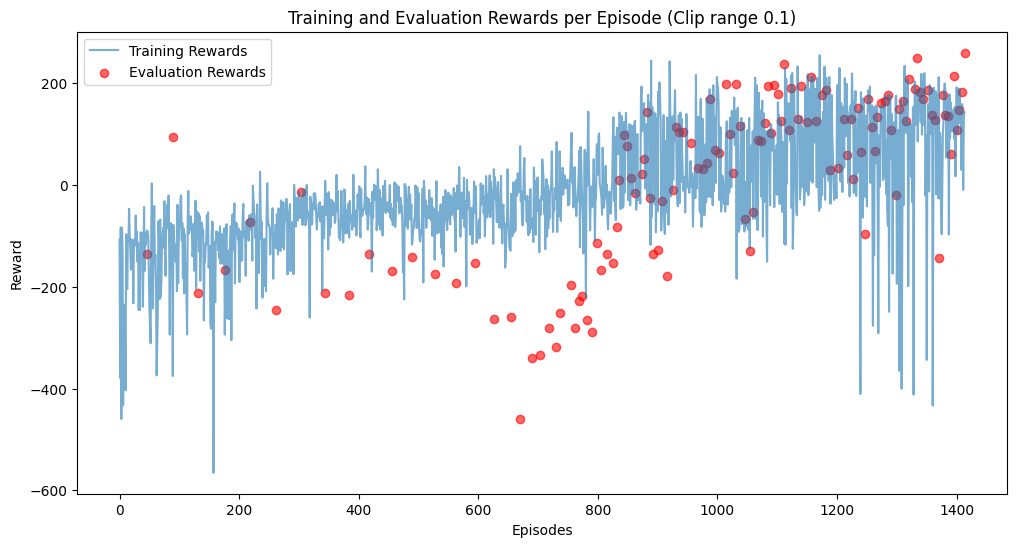
\includegraphics[width=\linewidth]{ppo_figures/cr_results_0.1.png}
				\caption{$\varepsilon=0.1$}
				\label{fig:ppo_cr01}
			\end{subfigure}\hfill 
			\begin{subfigure}{0.48\textwidth}
				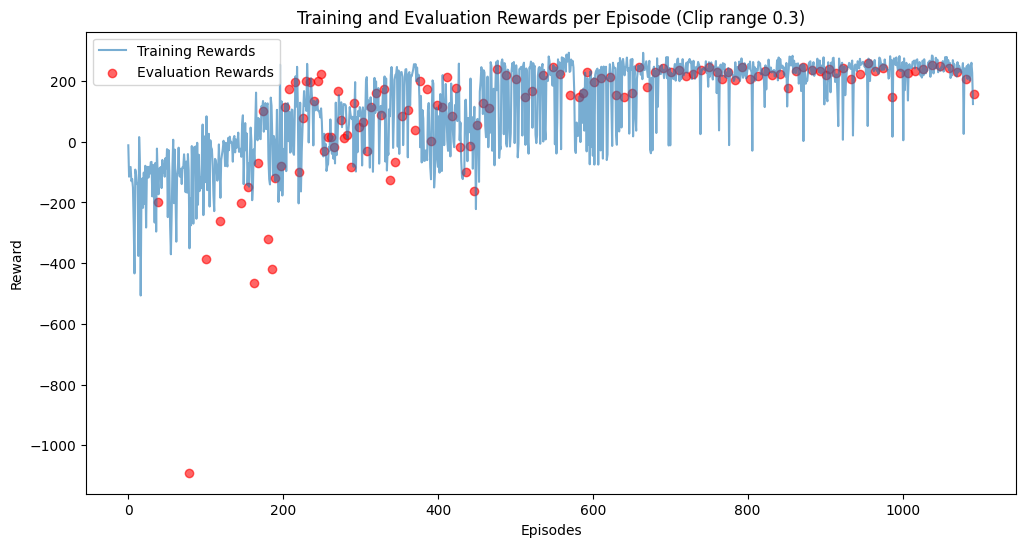
\includegraphics[width=\linewidth]{ppo_figures/cr_results_0.3.png}
				\caption{$\varepsilon=0.3$}
				\label{fig:ppo_cr03}
			\end{subfigure}\\ 
			\begin{subfigure}{0.48\textwidth}
				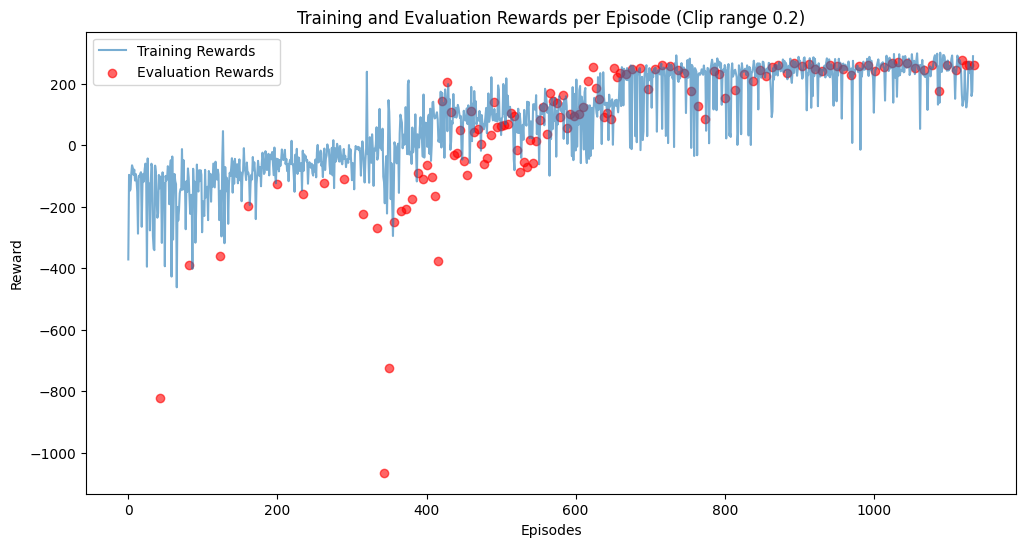
\includegraphics[width=\linewidth]{ppo_figures/cr_results_0.2.png}
				\caption{$\varepsilon=0.2$}
				\label{fig:ppo_cr02}
			\end{subfigure}\
		\end{center}
		\caption{Training and evaluation rewards of PPO for different clip rates $\varepsilon=0.1,0.2,0.3$}
		\label{fig:ppo_cliprate}
	\end{figure}
	
	Finally, we compare the performance of PPO on its salient clip value $\varepsilon$. $\varepsilon=0.2$ was the originally proposed default choice of the authors and proved optimal among our three candidates with regard to variance and convergence rate (Fig. \ref{fig:ppo_cr02}). While the agent still culminated in successful behaviour for $\varepsilon=0.3$, the mean rewards during evaluation clearly depict that the policy parameters oscillate more strongly, which we hypothesize to be attributable to the approximation error of the state distribution $P_{\pi_{\theta'}}$ because of the larger allowed distributional shift (Fig. \ref{fig:ppo_cr03}). On the contrary, the variance and performance of the policy aggravates for a smaller $\varepsilon=0.1$ too (Fig. \ref{fig:ppo_cr01}). We believe that the reason for this might be similar to the results observed for the low learning rate in Figure \ref{fig:ppo_lr0.0003}. The constraint might be so strong that it hinders the agent from escaping from local minima and reaching unseen and more desirable regions in the optimization landscape.
	\subsection{REINFORCE}
	\section{Conclusion}
	\bibliography{references.bib}
\end{document}